%\documentclass[smaller,handout]{beamer}
\documentclass[smaller]{beamer}

\usepackage{amsfonts}
\usepackage{amssymb}
\usepackage{amsmath}
\usepackage{mathtools}
\usepackage{epsfig}
\usepackage{graphicx}
\usepackage{rotating}

\def\F{{\cal F}}
\def\X{{\cal X}}
\def\Y{{\cal Y}}
\def\Z{{\cal Z}}
\def\P{{\mathbb P}}
\def\R{{\mathbb R}}
\def\E{{\mathbb E}}
\def\bZ{{\mathbb Z}}
\def\darkred{\color{red!70!black}}
\def\darkgreen{\color{green!60!black}}
\def\learn{{\mbox{LEARN}}}
\def\err{{\mbox{err}}}
\def\bI{{\tilde{I}}}
\def\dis{{\mbox{DIS}}}

\DeclareMathOperator*{\argmin}{arg\,min}
\DeclareMathOperator*{\argmax}{arg\,max}

%\usepackage{pgfpages}
%\pgfpagesuselayout{4 on 1}[letterpaper,border shrink=5mm,landscape]

%\usepackage{beamerarticle}

\mode<presentation>
{
  \usetheme{default}
%  \setbeamercovered{transparent}
  % or whatever (possibly just delete it)
}


\usepackage[english]{babel}
% or whatever

\useinnertheme{circles}
\usefonttheme{structurebold}

%\usepackage[latin1]{inputenc}
% or whatever

%\usepackage{times}
%\usepackage[T1]{fontenc}
% Or whatever. Note that the encoding and the font should match. If T1
% does not look nice, try deleting the line with the fontenc.

\title{Dimension Reduction using PCA and SVD}

\author{} %Sanjoy Dasgupta}
% - Give the names in the same order as the appear in the paper.
% - Use the \inst{?} command only if the authors have different
%   affiliation.

%\institute{University of California, San Diego}

\date{}

% If you wish to uncover everything in a step-wise fashion, uncomment
% the following command: 

%\beamerdefaultoverlayspecification{<+->}
\setbeamertemplate{navigation symbols}{}

\def\vone{{\vskip.1in}}
\def\v2{{\vskip.2in}}
\def\bR{{\mathbb R}}
\def\R{{\mathbb R}}
\def\eps{{\epsilon}}
\def\E{{\mathbb E}}
\def\epso{{\epsilon_o}}
\def\nicered{{\color{red!70!black}}}
\def\pr{{\mbox{\rm Pr}}}

\setbeamercolor{title}{fg=red!80!black,bg=red!20!white}
\setbeamercolor{author}{fg=blue!80!black}

\begin{document}

% *** TITLE ***
\begin{frame}
  \titlepage
\end{frame}

% *** DIMENSIONALITY REDUCTION ***
\begin{frame}
\frametitle{Plan of Class}
\begin{itemize}
\item Starting the machine Learning part of the course.
\item Based on Linear Algebra.
\item If your linear algebra is rusty, check out the pages on
  ``Resources/Linear Algebra''
\item This class will all be theory.
\item Next class will be on doing PCA in Spark.
\item HW3 will open on friday, be due the following friday.
\end{itemize}
\end{frame}
\begin{frame}
\frametitle{Dimensionality reduction}

{\darkred Why reduce the number of features in a data set?}
\begin{enumerate}
\item It reduces storage and computation time.
\item High-dimensional data often has a lot of redundancy.
\item Remove noisy or irrelevant features.
\end{enumerate}


\pause\v2
{\darkgreen Example: are all the pixels in an image equally
  informative?}

$28\times28 = 784$pixels. A vector $ \vec{x} \in \R^{784}$

\vone
\hskip.25in

\includegraphics[width=1in]{mnist1.jpg}
\hskip.25in
\raisebox{.25in}{\begin{minipage}[b]{2.5in}
\onslide<3->{If we were to choose a few pixels to discard, which would be the prime candidates?}

\vone
\onslide<4->{\alert{Those with lowest variance...}}
\end{minipage}}

\end{frame}

% *** ELIMINATING LOW VARIANCE COORDINATES ***
\begin{frame}
\frametitle{Eliminating low variance coordinates}

{\darkred Example: MNIST. What fraction of the total variance is contained in the 100 (or 200, or 300) coordinates with lowest variance?}

\pause\v2

\begin{center}
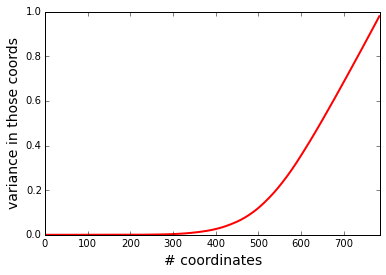
\includegraphics[width=3in]{mnistvar.png}
\end{center}

\pause
We can easily drop 300-400 pixels...

\pause
Can we eliminate more?

\pause
\alert{Yes! By using features that are {\bf combinations} of pixels instead of single pixels.}
\end{frame}

% *** COVARIANCE AND CORRELATION ***
\begin{frame}
\frametitle{Covariance (a quick review)}

{\darkred Suppose $X$ has mean $\mu_X$ and $Y$ has mean $\mu_Y$.}

\v2
\begin{itemize}
\item \alert{Covariance}
$$ \mbox{cov}(X,Y) = \E [(X-\mu_X)(Y-\mu_Y)] = \E[XY] - \mu_X \mu_Y $$
Maximized when $X=Y$, in which case it is $\mbox{var}(X)$. 

In general, it is at most $\mbox{std}(X) \mbox{std}(Y)$.

\end{itemize}

\end{frame}

% *** COVARIANCE AND CORRELATION: EXAMPLE 1 ***
\begin{frame}
\frametitle{Covariance: example 1}

\alert{
\begin{align*}
\mbox{cov}(X,Y) 
&= 
\E [(X-\mu_X)(Y-\mu_Y)] \ = \ \E [XY] - \mu_X \mu_Y
\end{align*}}

\begin{columns}
\begin{column}[b]{1.5in}
\raisebox{.75in}{
\hskip.5in
\begin{tabular}{ccc}
$x$ & $y$ & $\pr(x,y)$ \\ \hline
$-1$  & $-1$  &  $1/3$ \\ 
$-1$  &  $1$  &  $1/6$ \\
$1$   &  $-1$ &  $1/3$ \\
$1$   &  $1$  &  $1/6$
\end{tabular}}
\end{column}

\begin{column}[b]{3in}
\begin{align*}
\mu_X &= \onslide<2->{0} \\
\mu_Y &= \onslide<3->{-1/3} \\
\mbox{var}(X) &= \onslide<4->{1} \\
\mbox{var}(Y) &= \onslide<5->{8/9} \\
\mbox{cov}(X,Y) &= \onslide<6->{0} \\
\end{align*}
\end{column}
\end{columns}

\v2
\onslide<7->{\darkred
In this case, $X,Y$ are independent. 
Independent variables always have zero
covariance.}

\end{frame}

% *** COVARIANCE AND CORRELATION: EXAMPLE 2 ***
\begin{frame}
\frametitle{Covariance: example 2}

\alert{
\begin{align*}
\mbox{cov}(X,Y) 
&= 
\E [(X-\mu_X)(Y-\mu_Y)] \ = \ \E [XY] - \mu_X \mu_Y
\end{align*}}

\begin{columns}
\begin{column}[b]{1.5in}
\raisebox{.75in}{
\hskip.5in
\begin{tabular}{ccc}
$x$ & $y$ & $\pr(x,y)$ \\ \hline
$-1$  & $-10$  &  $1/6$ \\ 
$-1$  & $10$   &  $1/3$ \\
$1$   & $-10$  &  $1/3$ \\
$1$   & $10$   &  $1/6$
\end{tabular}}
\end{column}

\begin{column}[b]{3in}
\begin{align*}
\mu_X &= \onslide<2->{0} \\
\mu_Y &= \onslide<3->{0} \\
\mbox{var}(X) &= \onslide<4->{1} \\
\mbox{var}(Y) &= \onslide<5->{100} \\
\mbox{cov}(X,Y) &= \onslide<6->{-10/3}
\end{align*}
\end{column}
\end{columns}

\v2
\onslide<8->{\darkred
In this case, $X$ and $Y$ are negatively correlated.
\\
}
\end{frame}

% *** EXAMPLE: MNIST ***
\begin{frame}
\frametitle{Example: MNIST}

\hskip.1in

\includegraphics[width=1in]{mnist1.jpg}
\hskip.1in
\raisebox{.2in}{
\begin{minipage}[b]{2.8in}
{\darkgreen approximate a digit from class $j$ as the class average plus $k$
  corrections:}
$$
\vec{x} \approx \mu_j + \sum_{i=1}^k a_i \vec{v}_{j,i}
$$
\begin{itemize}
\item <2->{\darkgreen $\mu_j \in \R^{784}$} class mean vector
\item <3->{\darkgreen $\vec{v}_{j,1},\ldots,\vec{v}_{j,k}$} are the
  {\bf principal directions}.
\end{itemize}
\end{minipage}
}
\end{frame}

% *** THE EFFECT OF CORRELATION ***
\begin{frame}
\frametitle{The effect of correlation}

{\darkred Suppose we wanted just one feature for the following data.}

\v2
\begin{center}
\includegraphics<1>[width=2.5in]{corr1.png}
\includegraphics<2->[width=2.5in]{corr2.png}
\end{center}

\v2
\onslide<3->{\alert{This is the {\bf direction of maximum variance}.}}

\end{frame}


% *** TWO TYPES OF PROJECTION ***
\begin{frame}
\frametitle{Two types of projection}

\begin{center}
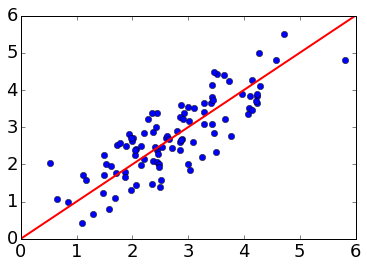
\includegraphics[width=1.75in]{corr2.png}
\end{center}

\begin{columns}
\begin{column}[t]{2in}

Projection onto $\R$:

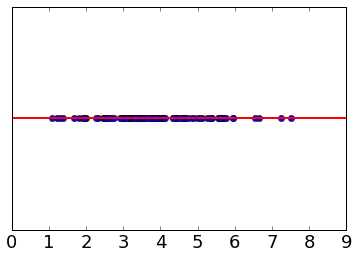
\includegraphics[width=1.75in]{corr3.png}
  
\end{column}
\begin{column}[t]{2in}

Projection onto a 1-d line in $\R^2$:

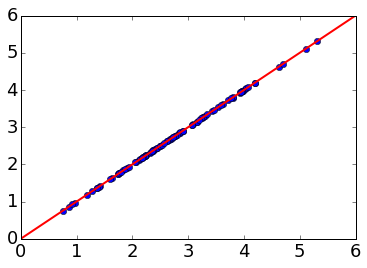
\includegraphics[width=1.75in]{corr4.png}

\end{column}
\end{columns}

\end{frame}

% *** PROJECTION: FORMALLY ***
\begin{frame}
\frametitle{Projection: formally}

{\darkred What is the projection of $x \in \R^p$ onto direction $u \in \R^p$ (where $\|u\| = 1$)?}

\v2
\hskip.25in
\includegraphics[width=1.25in]{proj.pdf}
\hskip.25in
\raisebox{0in}{\begin{minipage}[b]{2.5in}
\onslide<2->{
As a one-dimensional value: $$ x \cdot u = u \cdot x = u^T x = \sum_{i=1}^p u_i x_i .$$}
\onslide<3->{As a $p$-dimensional vector: $$ (x \cdot u) u = uu^T x $$
``Move $x \cdot u$ units in direction $u$''}
\end{minipage}}

\v2
\onslide<4->{{\darkgreen What is the projection of $x = \begin{pmatrix} 2 \\ 3 \end{pmatrix}$ onto the following directions?}}
\begin{itemize}
\item<5-> {\darkgreen The coordinate direction $e_1$?} \onslide<6->{\ \ Answer: $2$}
\item<7-> {\darkgreen The direction $\begin{pmatrix} 1 \\ -1 \end{pmatrix}$?} \onslide<8->{\ \ Answer: $-1/\sqrt{2}$}
\end{itemize}

\end{frame}

% *** Matrix Notation ***

\begin{frame}
\frametitle{matrix notation I }

{\darkred A notation that allows a simple representation of multiple projections}

\pause\vone
A vector $\vec{v} \in \R^d$ can be represented, in matrix
  notation, as
\begin{itemize}
\item A column vector: $$v= \begin{pmatrix} v_1 \\ v_2 \\ \vdots \\  v_d \end{pmatrix}$$
\item A row vector: $$v^T=\begin{pmatrix} v_1 & v_2 &\cdots&  v_d \end{pmatrix}$$
\end{itemize}
\end{frame}

\begin{frame}
\frametitle{matrix notation II}

\pause \vone
By convension an {\darkred inner} product is represented by a {\bf row} vector
followed by a a {\bf column} vector:
$$
\begin{pmatrix} u_1 & u_2 &\cdots& u_d \end{pmatrix} \begin{pmatrix} v_1
  \\ v_2 \\ \vdots \\
  v_d \end{pmatrix} = \sum_{i=1}^d u_i v_i
$$

\pause \vone
While a {\bf column} vector followd by a {\bf row} vector represents
an {\darkred outer} product which is a matrix: 
$$ 
\begin{pmatrix} v_1  \\ v_2 \\ \vdots \\  v_n \end{pmatrix} 
\begin{pmatrix} u_1 & u_2 &\cdots& u_m \end{pmatrix}  =
\begin{pmatrix}
u_1 v_1 & u_2 v_1 & \cdots & u_m v_1 \\
\vdots & \ddots & \ddots & \vdots \\
u_1 v_n & u_2 v_n & \cdots & u_m v_n
\end{pmatrix}
$$


\end{frame}

% *** PROJECTION ONTO MULTIPLE DIRECTIONS ***
\begin{frame}
\frametitle{Projection onto multiple directions}

{\darkred Want to project $x \in \R^p$ into the $k$-dimensional subspace defined by vectors $u_1, \ldots, u_k \in \R^p$.}

\pause\vone
This is easiest when the $u_i$'s are {\bf orthonormal}:
\begin{itemize}
\item They each have length one.
\item They are at right angles to each other: $u_i \cdot u_j = 0$ whenever $i \neq j$
\end{itemize}

\pause\vone
Then the projection, as a $k$-dimensional vector, is
$$ (x \cdot u_1, x \cdot u_2, \ldots, x \cdot u_k)
\ = \ 
\underbrace{\begin{pmatrix} 
\xleftarrow{\hspace*{1cm}} u_1 \xrightarrow{\hspace*{1cm}} \\
\xleftarrow{\hspace*{1cm}} u_2 \xrightarrow{\hspace*{1cm}} \\
 \vdots \\ 
\xleftarrow{\hspace*{1cm}} u_k \xrightarrow{\hspace*{1cm}} 
\end{pmatrix}}_{\text{call this $U^T$}} 
\begin{pmatrix}
\Big\uparrow \\
x \\
\Big\downarrow
\end{pmatrix}
$$

\pause\vone
{\darkgreen As a $p$-dimensional vector, the projection is
$$ (x \cdot u_1) u_1 + (x \cdot u_2) u_2 + \cdots + (x \cdot u_k)u_k = UU^T x.$$}
\end{frame}

% *** PROJECTION ONTO MULTIPLE DIRECTIONS: EXAMPLE ***
\begin{frame}
\frametitle{Projection onto multiple directions: example}

{\darkred Suppose data are in $\R^4$ and we want to project onto the first two coordinates.} 

\vskip-.2in
\begin{flalign*} 
\onslide<2->{& \mbox{Take vectors\ \ \ \ } 
u_1 = \begin{pmatrix} 1 \\ 0 \\ 0 \\ 0 \end{pmatrix}, \ \ \ 
u_2 = \begin{pmatrix} 0 \\ 1 \\ 0 \\ 0 \end{pmatrix} 
\mbox{\ \ \ \ (notice: orthonormal)} & \\}
\onslide<3->{
&\mbox{Then write \ \ \ \ } U^T \ = \ 
\begin{pmatrix}
\xleftarrow{\hspace*{1cm}} u_1 \xrightarrow{\hspace*{1cm}} \\
\xleftarrow{\hspace*{1cm}} u_2 \xrightarrow{\hspace*{1cm}} 
\end{pmatrix}
\ = \ 
\begin{pmatrix}
1 & 0 & 0 & 0 \\
0 & 1 & 0 & 0
\end{pmatrix}&}
\end{flalign*}

\v2
\begin{columns}
\begin{column}[t]{1.5in}
\onslide<4->{\darkgreen The projection of $x\in \R^4$, as a 2-d vector, is
$$ U^Tx = \begin{pmatrix} x_1 \\ x_2\end{pmatrix} $$}
\end{column}
\begin{column}[t]{1.5in}
\onslide<5->{\darkgreen The projection of $x$ as a 4-d vector is
$$ UU^T x = \begin{pmatrix} x_1 \\ x_2 \\ 0 \\ 0 \end{pmatrix}$$}
\end{column}
\end{columns}

\onslide<6->{\alert{But we'll generally project along non-coordinate directions.}}
\end{frame}

% *** THE BEST SINGLE DIRECTION *** 
\begin{frame}
\frametitle{The best single direction}

{\darkred Suppose we need to map our data $x \in \R^p$ into just {\bf one} dimension:
$$ x \mapsto u \cdot x \mbox{\ \ \ \ for some unit direction $u \in \R^p$} $$
What is the direction $u$ of maximum variance?}

\pause\vone
\alert{{\bf Theorem}: Let $\Sigma$ be the $p \times p$ covariance matrix of $X$. 
The variance of $X$ in direction $u$ is given by $u^T \Sigma u$.}
\begin{itemize}
\item<3-> Suppose the mean of $X$ is $\mu \in \R^p$. The projection $u^T X$ has mean
$$ \E (u^T X) = u^T \E X = u^T \mu .$$
\item<4-> The variance of $u^T X$ is
\begin{align*}
\mbox{var}(u^T X) &= \E (u^TX - u^T \mu)^2 = \E (u^T (X-\mu)(X-\mu)^T u) \\
&= u^T \E (X-\mu)(X-\mu)^T u = u^T \Sigma u .
\end{align*}
\end{itemize}

\onslide<5->{\darkgreen Another theorem: $u^T \Sigma u$ is maximized by setting $u$ to the first {\bf eigenvector} of $\Sigma$. The maximum value is the corresponding {\bf eigenvalue}.}

\end{frame}

% *** BEST SINGLE DIRECTION: EXAMPLE ***
\begin{frame}
\frametitle{Best single direction: example}

\begin{center}
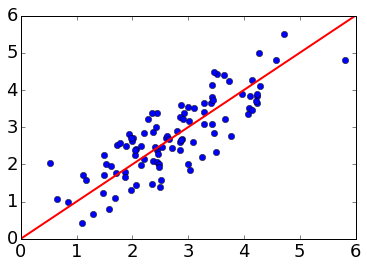
\includegraphics[width=2.5in]{corr2.png}
\end{center}

\v2
This direction is the {\bf first eigenvector} of the $2 \times 2$ covariance matrix of the data.

\end{frame}

% *** THE BEST K-DIMENSIONAL PROJECTION ***
\begin{frame}
\frametitle{The best $k$-dimensional projection}

Let $\Sigma$ be the $p \times p$ covariance matrix of $X$. Its {\bf eigendecomposition} 
can be computed in $O(p^3)$ time and consists of:
\begin{itemize}
\item real {\bf eigenvalues} $\lambda_1 \geq \lambda_2 \geq \cdots \geq \lambda_p$
\item corresponding {\bf eigenvectors} $u_1, \ldots, u_p \in \R^p$ that are orthonormal: that is, each $u_i$ has unit length and $u_i \cdot u_j = 0$ whenever $i \neq j$.
\end{itemize}

\pause\v2
{\darkred {\bf Theorem}: Suppose we want to map data $X \in \R^p$ to just $k$ dimensions,
while capturing as much of the variance of $X$ as possible. The best choice of 
projection is:
$$ x \mapsto (u_1 \cdot x, u_2 \cdot x, \ldots, u_k \cdot x),$$
where $u_i$ are the eigenvectors described above.}

\pause\v2
\alert{Projecting the data in this way is {\bf principal component analysis} (PCA).}

\end{frame}

% *** EXAMPLE: MNIST ***
\begin{frame}
\frametitle{Example: MNIST}

Contrast coordinate projections with PCA:

\begin{center}
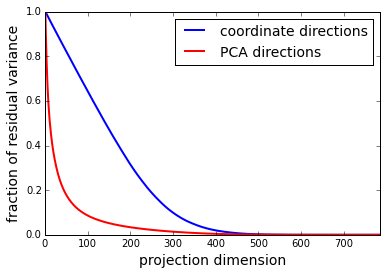
\includegraphics[width=3in]{mnist-compare.png}
\end{center}

\end{frame}

% *** MNIST: IMAGE RECONSTRUCTION ***
\begin{frame}
\frametitle{MNIST: image reconstruction}

\hskip.25in

\includegraphics[width=1.25in]{mnist2.png}
\hskip.25in
\raisebox{.5in}{\begin{minipage}[b]{2.5in}
{\darkred Reconstruct this original image from its PCA projection
to $k$ dimensions.}
\end{minipage}}

\pause\vone

\begin{tabular}{cccc}
{\darkgreen $k = 200$} & 
{\darkgreen $k = 150$} & 
{\darkgreen $k = 100$} & 
{\darkgreen $k = 50$} \\

\includegraphics[width=0.9in]{mnist2-200.png} &

\includegraphics[width=0.9in]{mnist2-150.png} &

\includegraphics[width=0.9in]{mnist2-100.png} &

\includegraphics[width=0.9in]{mnist2-50.png}
\end{tabular}

\pause\vone
\alert{Q: What are these reconstructions exactly?}

\pause
\alert{A: Image $x$ is reconstructed as $UU^Tx$, where $U$ is a $p \times k$ matrix whose columns are the top $k$ eigenvectors of $\Sigma$.}

\end{frame}

% *** WHAT ARE EIGENVALUES AND EIGENVECTORS? ***
\begin{frame}
\frametitle{What are eigenvalues and eigenvectors?}

{\darkgreen There are several steps to understanding these.}
\begin{enumerate}
\item<2-> Any matrix $M$ defines a function (or {\bf transformation}) $x \mapsto Mx$.
\item<3-> If $M$ is a $p \times q$ matrix, then this transformation maps vector $x \in \R^q$ to vector $Mx \in \R^p$.
\item<4-> We call it a {\bf linear transformation} because $M(x + x') = Mx + Mx'$.
\item<5-> We'd like to understand the nature of these transformations. The easiest case is when $M$ is {\bf diagonal}:
$$
\underbrace{\begin{pmatrix}
2 & 0 & 0 \\
0 & -1 & 0 \\
0 & 0 & 10
\end{pmatrix}}_{M}
\underbrace{\begin{pmatrix} x_1 \\ x_2 \\ x_3 \end{pmatrix}}_{x}
\ \ = \ \ 
\underbrace{\begin{pmatrix} 2x_1 \\ -x_2 \\ 10x_3 \end{pmatrix}}_{Mx}
$$
In this case, $M$ simply scales each coordinate separately.
\item<6-> What about more general matrices that are symmetric but not necessarily diagonal? They also just scale coordinates separately, but in a {\bf different coordinate system}.
\end{enumerate}
\end{frame}

% *** EIGENVALUE AND EIGENVECTOR: DEFINITION ***
\begin{frame}
\frametitle{Eigenvalue and eigenvector: definition}

{\darkred 
Let $M$ be a $p \times p$ matrix. 

We say $u \in \R^p$ is an {\bf eigenvector} if $M$ maps $u$ onto the same direction, that is,
$$ Mu = \lambda u$$
for some scaling constant $\lambda$. This $\lambda$ is the {\bf eigenvalue} associated with $u$.}

\pause\v2
Question: What are the eigenvectors and eigenvalues of:
$$ M = \begin{pmatrix}
2 & 0 & 0 \\
0 & -1 & 0 \\
0 & 0 & 10
\end{pmatrix} \ ?
$$

\pause
Answer: Eigenvectors $e_1, e_2. e_3$, with corresponding eigenvalues $2,-1,10$.

\pause\v2
\alert{Notice that these eigenvectors form an orthonormal basis.}
\end{frame}

% *** EIGENVECTORS OF A REAL SYMMETRIC MATRIX ***
\begin{frame}
\frametitle{Eigenvectors of a real symmetric matrix}

{\bf Theorem.} Let $M$ be any real symmetric $p \times p$ matrix. Then $M$ has
\begin{itemize}
\item $p$ eigenvalues $\lambda_1, \ldots, \lambda_p$
\item corresponding eigenvectors $u_1, \ldots, u_p \in \R^p$ that are orthonormal
\end{itemize}

\pause\v2
\alert{We can think of $u_1, \ldots, u_p$ as being the axes of the natural coordinate 
system for understanding $M$.}

\pause\v2
{\darkgreen Example: consider the matrix
$$ M = \begin{pmatrix} 3 & 1 \\ 1 & 3 \end{pmatrix} $$
It has eigenvectors
$$ u_1 = \frac{1}{\sqrt{2}} \begin{pmatrix} 1 \\ 1 \end{pmatrix}, \ \ \ 
u_2 = \frac{1}{\sqrt{2}} \begin{pmatrix} -1 \\ 1 \end{pmatrix} $$
and corresponding eigenvalues $\lambda_1 = 4$ and $\lambda_2 = 2$. (Check)}
\end{frame}

% *** SPECTRAL DECOMPOSITION ***
\begin{frame}
\frametitle{Spectral decomposition}

{\bf Theorem.} Let $M$ be any real symmetric $p \times p$ matrix. Then $M$ has
\begin{itemize}
\item $p$ eigenvalues $\lambda_1, \ldots, \lambda_p$
\item corresponding eigenvectors $u_1, \ldots, u_p \in \R^p$ that are orthonormal
\end{itemize}

\pause\v2
{\darkred
{\bf Spectral decomposition:} Here is another way to write $M$:
$$ 
M = 
\underbrace{\begin{pmatrix}
\Big\uparrow   & \Big\uparrow   &         & \Big\uparrow \\
u_1            & u_2            &  \cdots & u_p  \\
\Big\downarrow & \Big\downarrow &         & \Big\downarrow
\end{pmatrix}}_{\text{$U$: columns are eigenvectors}}
\underbrace{\begin{pmatrix}
\lambda_1 &      0    & \cdots & 0      \\
0         & \lambda_2 & \cdots & 0      \\
\vdots    &   \vdots  & \ddots & \vdots \\
0         &     0     & \cdots & \lambda_p
\end{pmatrix}}_{\text{$\Lambda$: eigenvalues on diagonal}}
\underbrace{\begin{pmatrix} 
\xleftarrow{\hspace*{1cm}} u_1 \xrightarrow{\hspace*{1cm}} \\
\xleftarrow{\hspace*{1cm}} u_2 \xrightarrow{\hspace*{1cm}} \\
 \vdots \\ 
\xleftarrow{\hspace*{1cm}} u_p \xrightarrow{\hspace*{1cm}} 
\end{pmatrix}}_{U^T}
$$}
\pause
Thus $Mx = U\Lambda U^T x$, which can be interpreted as follows:
\begin{itemize}
\item $U^T$ rewrites $x$ in the $\{u_i\}$ coordinate system
\item $\Lambda$ is a simple coordinate scaling in that basis
\item $U$ then sends the scaled vector back into the usual coordinate basis
\end{itemize}
\end{frame}

% *** SPECTRAL DECOMPOSITION: EXAMPLE ***
\begin{frame}
\frametitle{Spectral decomposition: example}

{\darkgreen Apply spectral decomposition to the matrix $M$ we saw earlier:}
{\darkred $$ M = 
\begin{pmatrix} 3 & 1 \\ 1 & 3 \end{pmatrix} \
=
\underbrace{\frac{1}{\sqrt{2}}\begin{pmatrix} 1 & -1 \\ 1 & 1 \end{pmatrix}}_{U}
\underbrace{\begin{pmatrix} 4 & 0 \\ 0 & 2 \end{pmatrix}}_{\Lambda}
\underbrace{\frac{1}{\sqrt{2}}\begin{pmatrix} 1 & 1 \\ -1 & 1 \end{pmatrix}}_{U^T}
$$}

\raisebox{2in}{
\begin{minipage}[t]{1.25in}
  \begin{align*}
    \onslide<2->{M \begin{pmatrix} 1 \\ 2 \end{pmatrix}}
    \only<2>{&= \mbox{???} \\}
    \onslide<3->{&= U \Lambda U^T \begin{pmatrix}1 \\ 2 \end{pmatrix} \\}
    \onslide<6->{&= U \Lambda \frac{1}{\sqrt{2}} \begin{pmatrix} 3 \\ 1 \end{pmatrix} \\}
    \onslide<7->{&= U \frac{1}{\sqrt{2}} \begin{pmatrix} 12 \\ 2 \end{pmatrix} \\
    &= \begin{pmatrix} 5 \\ 7 \end{pmatrix}}
  \end{align*}
\end{minipage}}
\hskip.25in
\includegraphics<2-3>[width=2.5in]{basis-change-1.pdf}
\includegraphics<4>[width=2.5in]{basis-change-2.pdf}
\includegraphics<5->[width=2.5in]{basis-change-3.pdf}  

\end{frame}

% *** PRINCIPAL COMPONENT ANALYSIS: RECAP ***
\begin{frame}
  \frametitle{Principal component analysis: recap}

  {\darkgreen Consider data vectors $X \in \R^p$.}
  \begin{itemize}
  \item<2-> The covariance matrix $\Sigma$ is a $p \times p$ symmetric matrix.
  \item<3-> Get eigenvalues $\lambda_1 \geq \lambda_2 \geq \cdots \geq \lambda_p$, eigenvectors $u_1, \ldots, u_p$.
  \item<4-> $u_1, \ldots, u_p$ is an alternative basis in which to represent the data.
    \item<4-> The variance of $X$ in direction $u_i$ is $\lambda_i$.
  \item<5-> To project to $k$ dimensions while losing as little as possible of the overall variance, use
    $x \mapsto (x \cdot u_1, \ldots, x \cdot u_k)$.
  \end{itemize}

  \hskip.25in
      \includegraphics<1>[width=2in]{pca3.pdf}
    \includegraphics<2-3>[width=2in]{pca2.pdf}
    \includegraphics<4->[width=2in]{pca1.pdf}
    \hskip.25in
    \raisebox{.75in}{\begin{minipage}[t]{1.5in}
  \vskip-.2in
  \onslide<6->{\alert{What is the covariance of the projected data?}}
    \end{minipage}}
    

  
\end{frame}

% *** EXAMPLE: PERSONALITY ASSESSMENT ***
\begin{frame}
\frametitle{Example: personality assessment}

\alert{What are the dimensions along which personalities differ?}
\begin{itemize}
\item<2-> {\it Lexical hypothesis}: most important personality characteristics have become encoded in natural language.
\item<3-> Allport and Odbert (1936): sat down with the English dictionary and extracted all terms that could be used to distinguish one person's behavior from another's. Roughly 18000 words, of which 4500 could be described as personality traits.
\item<4-> Step: group these words into (approximate) synonyms. This is done by manual clustering. e.g. Norman (1967):

\begin{center}
\includegraphics[width=2in]{norman1.pdf}
\end{center}

\item<5-> Data collection: Ask a variety of subjects to what extent each of these words describes them.
\end{itemize}
\end{frame}

% *** PERSONALITY ASSESSMENT: THE DATA ***
\begin{frame}
\frametitle{Personality assessment: the data}

{\darkred Matrix of data (1 = strongly disagree, 5 = strongly agree)}

\vspace{.5in}

{\darkgreen
\begin{center}
\begin{tabular}{l|cccccc}
& \begin{rotate}{60} shy \end{rotate} 
& \begin{rotate}{60} merry \end{rotate} 
& \begin{rotate}{60} tense \end{rotate} 
& \begin{rotate}{60} boastful \end{rotate} 
& \begin{rotate}{60} forgiving \end{rotate} 
& \begin{rotate}{60} quiet \end{rotate} \\ \hline
Person 1 & 4 & 1 & 1 & 2 & 5 & 5 \\
Person 2 & 1 & 4 & 4 & 5 & 2 & 1 \\
Person 3 & 2 & 4 & 5 & 4 & 2 & 2 \\
         &       & \vdots &  &   
\end{tabular}
\end{center}}

How to extract important directions?

\pause
\begin{itemize}
\item Treat each column as a data point, find tight clusters
\item Treat each row as a data point, apply PCA
\item Other ideas: factor analysis, independent component analysis, ...
\end{itemize}

\pause\vone\alert{Many of these yield similar results}

\end{frame}

% *** WHAT DOES PCA ACCOMPLISH? ***
\begin{frame}
\frametitle{What does PCA accomplish?}

Example: suppose two traits (generosity, trust) are highly correlated, to the point where each person either answers ``1'' to both or ``5'' to both.

\begin{center}
\includegraphics<1>[width=2.5in]{personality-axes-1.pdf}
\includegraphics<2->[width=2.5in]{personality-axes-2.pdf}
\end{center}

\onslide<3->{\alert{This single PCA dimension entirely accounts for the two traits.}}

\end{frame}

% *** THE BIG FIVE TAXONOMY ***
\begin{frame}
\frametitle{The ``Big Five'' taxonomy}

\includegraphics[width=4.25in]{bigfive.pdf}

\pause\v2
\alert{Many applications, such as online match-making.}

\end{frame}

% *** SINGULAR VALUE DECOMPOSITION (SVD) ***
\begin{frame}
\frametitle{Singular value decomposition (SVD)}

For {\bf symmetric} matrices, such as covariance matrices, we have seen:
\begin{itemize}
\item Results about existence of eigenvalues and eigenvectors
\item The fact that the eigenvectors form an alternative basis
\item The resulting spectral decomposition, which is used in PCA
\end{itemize}
But what about arbitrary matrices $M \in \R^{p \times q}$? 

\pause\v2
\alert{Any $p \times q$ matrix (say $p \leq q$) has a {\bf singular value decomposition}:}
{\darkred 
$$
M = 
\underbrace{\begin{pmatrix}
\big\uparrow    &         & \big\uparrow \\[.05in]
u_1             &  \cdots  & u_p  \\[.05in]
\big\downarrow  &         & \big\downarrow
\end{pmatrix}}_{\text{$p \times p$ matrix $U$}}
\underbrace{\begin{pmatrix}
\sigma_1  & \cdots & 0       \\
\vdots    & \ddots & \vdots  \\
0         & \cdots & \sigma_p            
\end{pmatrix}}_{\text{$p \times p$ matrix $\Lambda$}}
\underbrace{\begin{pmatrix} 
\xleftarrow{\hspace*{1cm}} v_1 \xrightarrow{\hspace*{1cm}} \\
\vdots \\
\xleftarrow{\hspace*{1cm}} v_p \xrightarrow{\hspace*{1cm}} 
\end{pmatrix}}_{\text{$p\times q$ matrix $V^T$}}
$$}
\begin{itemize}
\item {\darkgreen $u_1, \ldots, u_p$ are orthonormal vectors in $\R^p$}
\item {\darkgreen $v_1, \ldots, v_p$ are orthonormal vectors in $\R^q$}
\item {\darkgreen $\sigma_1 \geq \sigma_2 \geq \cdots \geq \sigma_p$ are {\bf singular values}}
\end{itemize}

\end{frame}

% *** MATRIX APPROXIMATION ***
\begin{frame}
\frametitle{Matrix approximation}

We can {\bf factor} any $p \times q$ matrix as $M = UW^T$:
\begin{align*}
M
&= 
\begin{pmatrix}
\big\uparrow    &         & \big\uparrow \\[.05in]
u_1             &  \cdots & u_p  \\[.05in]
\big\downarrow  &         & \big\downarrow
\end{pmatrix}
\begin{pmatrix}
\sigma_1  & \cdots & 0       \\
\vdots    & \ddots & \vdots  \\
0         & \cdots & \sigma_p            
\end{pmatrix}
\begin{pmatrix} 
\xleftarrow{\hspace*{1cm}} v_1 \xrightarrow{\hspace*{1cm}} \\
\vdots \\
\xleftarrow{\hspace*{1cm}} v_p \xrightarrow{\hspace*{1cm}} 
\end{pmatrix} \\
&=
\underbrace{\begin{pmatrix}
\big\uparrow    &         & \big\uparrow \\[.05in]
u_1             &  \cdots & u_p  \\[.05in]
\big\downarrow  &         & \big\downarrow
\end{pmatrix}}_{\text{$p \times p$ matrix $U$}}
\underbrace{\begin{pmatrix} 
\xleftarrow{\hspace*{1cm}} \sigma_1 v_1 \xrightarrow{\hspace*{1cm}} \\
\vdots \\
\xleftarrow{\hspace*{1cm}} \sigma_p v_p \xrightarrow{\hspace*{1cm}} 
\end{pmatrix}}_{\text{$p \times q$ matrix $W^T$}}
\end{align*}

\pause
{\darkred A concise approximation to $M$: just take the first $k$ columns of $U$ and the first $k$ rows of $W^T$, for $k < p$:
$$
\widehat{M} =
\underbrace{\begin{pmatrix}
\big\uparrow    &         & \big\uparrow \\[.05in]
u_1             &  \hskip-.2in\cdots\hskip-.2in & u_k  \\[.05in]
\big\downarrow  &         & \big\downarrow
\end{pmatrix}}_{p \times k}
\underbrace{\begin{pmatrix} 
\xleftarrow{\hspace*{1cm}} \sigma_1 v_1 \xrightarrow{\hspace*{1cm}} \\[-.05in]
\vdots \\[-0.05in]
\xleftarrow{\hspace*{1cm}} \sigma_k v_k \xrightarrow{\hspace*{1cm}} 
\end{pmatrix}}_{k \times q}
$$}

\end{frame}

% *** EXAMPLE: TOPIC MODELING ***
\begin{frame}
\frametitle{Example: topic modeling}

{\darkgreen Blei (2012):}

\vone

\includegraphics[width=4.25in]{topic.pdf}

\end{frame}

% *** LATENT SEMANTIC INDEXING ***
\begin{frame}
\frametitle{Latent semantic indexing (LSI)}

Given a large corpus of $n$ documents:
\begin{itemize}
\item Fix a vocabulary, say of $V$ words.
\item Bag-of-words representation for documents: each document becomes a vector of length $V$, with one coordinate per word.
\item The corpus is an $n \times V$ matrix, one row per document.
\end{itemize}

\vskip.5in
{\darkgreen 
\begin{center}
\begin{tabular}{l|cccccc}
& \begin{rotate}{60} cat \end{rotate} 
& \begin{rotate}{60} dog \end{rotate} 
& \begin{rotate}{60} house \end{rotate} 
& \begin{rotate}{60} boat \end{rotate} 
& \begin{rotate}{60} garden \end{rotate} 
& $\cdots$ \\ \hline
Doc 1 & 4 & 1 & 1 & 0 & 2 &  \\
Doc 2 & 0 & 0 & 3 & 1 & 0 & \\
Doc 3 & 0 & 1 & 3 & 0 & 0 &  \\
         &       & \vdots &  &   
\end{tabular}
\end{center}}

\pause\v2
\alert{Let's find a concise approximation to this matrix $M$.}
\end{frame}

% *** LATENT SEMANTIC INDEXING, CONT'D ***
\begin{frame}
\frametitle{Latent semantic indexing, cont'd}

{\darkred Use SVD to get an approximation to $M$: for small $k$,}
$$
\underbrace{\begin{pmatrix} 
\xleftarrow{\hspace*{.5cm}} \text{doc 1} \xrightarrow{\hspace*{.5cm}} \\
\xleftarrow{\hspace*{.5cm}} \text{doc 2} \xrightarrow{\hspace*{.5cm}} \\
\xleftarrow{\hspace*{.5cm}} \text{doc 3} \xrightarrow{\hspace*{.5cm}} \\
\vdots \\
\xleftarrow{\hspace*{.5cm}} \text{doc $n$} \xrightarrow{\hspace*{.5cm}} 
\end{pmatrix}}_{\text{$n \times V$ matrix $M$}}
\ \approx \ 
\underbrace{\begin{pmatrix}
\xleftarrow{\hspace*{0.5cm}} \theta_1 \xrightarrow{\hspace*{0.5cm}} \\
\xleftarrow{\hspace*{0.5cm}} \theta_2 \xrightarrow{\hspace*{0.5cm}} \\
\xleftarrow{\hspace*{0.5cm}} \theta_3 \xrightarrow{\hspace*{0.5cm}} \\
\vdots \\
\xleftarrow{\hspace*{0.5cm}} \theta_n \xrightarrow{\hspace*{0.5cm}} 
\end{pmatrix}}_{\text{$n \times k$ matrix $\Theta$}}
\underbrace{\begin{pmatrix} 
\xleftarrow{\hspace*{1cm}} \Psi_1 \xrightarrow{\hspace*{1cm}} \\[-.05in]
\vdots \  \\
\xleftarrow{\hspace*{1cm}} \Psi_k \xrightarrow{\hspace*{1cm}} 
\end{pmatrix}}_{\text{$k \times V$ matrix $\Psi$}}
$$

\pause
{\darkred Think of this as a {\it topic model} with $k$ topics.}
\begin{itemize}
\item $\Psi_j$ is a vector of length $V$ describing topic $j$: coefficient $\Psi_{jw}$ is large if word $w$ appears often in that topic.
\item Each document is a combination of topics: $\theta_{ij}$ is the weight of topic $j$ in document $i$.
\end{itemize}

\pause\vone
\alert{Document $i$ originally represented by $i$th row of $M$, a vector in $\R^V$.

Can instead use $\theta_i \in \R^k$, a more concise ``semantic'' representation.}

\end{frame}

% *** THE RANK OF A MATRIX ***
\begin{frame}
\frametitle{The rank of a matrix}

{\darkred Suppose we want to approximate a matrix $M$ by a simpler matrix $\widehat{M}$. What is a suitable notion of ``simple''?}
\pause
\begin{itemize}
\item Let's say $M$ and $\widehat{M}$ are $p \times q$, where $p \leq q$.
\item Treat each row of $\widehat{M}$ as a data point in $\R^q$.
\item We can think of the data as ``simple'' if it actually lies in a low-dimensional subspace.
\item If the rows lie in $k$-dimensional subspace, we say that $\widehat{M}$ has {\bf rank} $k$.
\end{itemize}
\pause
\alert{The {\bf rank} of a matrix is the number of linearly independent rows.}

\pause\v2
{\darkred {\bf Low-rank approximation}: given $M \in \R^{p \times q}$ and an integer $k$, find the matrix $\widehat{M} \in \R^{p \times q}$ that is the best rank-$k$ approximation to $M$.} 

\pause\vone
That is, find $\widehat{M}$ so that
\begin{itemize}
\item $\widehat{M}$ has rank $\leq k$
\item The approximation error
$ \sum_{i,j} (M_{ij} - \widehat{M}_{ij})^2$
is minimized.
\end{itemize}

\pause
\alert{We can get $\widehat{M}$ directly from the singular value decomposition of $M$.}
\end{frame}



% *** LOW-RANK APPROXIMATION ***
\begin{frame}
\frametitle{Low-rank approximation}

Recall: Singular value decomposition of $p \times q$ matrix $M$ (with $p \leq q$): 
$$
M = 
\begin{pmatrix}
\big\uparrow    &         & \big\uparrow \\[.05in]
u_1             &  \cdots & u_p  \\[.05in]
\big\downarrow  &         & \big\downarrow
\end{pmatrix}
\begin{pmatrix}
\sigma_1  & \cdots & 0       \\
\vdots    & \ddots & \vdots  \\
0         & \cdots & \sigma_p            
\end{pmatrix}
\begin{pmatrix} 
\xleftarrow{\hspace*{1cm}} v_1 \xrightarrow{\hspace*{1cm}} \\
\vdots \\
\xleftarrow{\hspace*{1cm}} v_p \xrightarrow{\hspace*{1cm}} 
\end{pmatrix}
$$
\begin{itemize}
\item {\darkgreen $u_1, \ldots, u_p$ is an orthonormal basis of $\R^p$}
\item {\darkgreen $v_1, \ldots, v_q$ is an orthonormal basis of $\R^q$}
\item {\darkgreen $\sigma_1 \geq \cdots \geq \sigma_p$ are {\bf singular values}}
\end{itemize}

\pause\v2
{\darkred The {\bf best rank-$k$ approximation} to $M$, for any $k \leq p$, is then
$$
\widehat{M} = 
\underbrace{\begin{pmatrix}
\big\uparrow    &         & \big\uparrow \\
u_1             &  \hskip-.2in\cdots\hskip-.2in & u_k  \\
\big\downarrow  &         & \big\downarrow
\end{pmatrix}}_{\text{$p \times k$}}
\underbrace{\begin{pmatrix}
\sigma_1  & \hskip-.07in\cdots\hskip-.07in & 0       \\[-0.05in]
\vdots    & \hskip-.07in\ddots\hskip-.07in & \vdots  \\[-0.05in]
0         & \hskip-.07in\cdots\hskip-.07in & \sigma_k 
\end{pmatrix}}_{\text{$k \times k$}}
\underbrace{\begin{pmatrix} 
\xleftarrow{\hspace*{1cm}} v_1 \xrightarrow{\hspace*{1cm}} \\[-0.05in]
\vdots \\[-0.05in]
\xleftarrow{\hspace*{1cm}} v_k \xrightarrow{\hspace*{1cm}} \\
\end{pmatrix}}_{\text{$k\times q$}}
$$}
\end{frame}

% *** EXAMPLE: COLLABORATIVE FILTERING ***
\begin{frame}
\frametitle{Example: Collaborative filtering}

{\darkgreen Details and images from Koren, Bell, Volinksy (2009).}

\v2
{\bf Recommender systems}: matching customers with products.
\begin{itemize}
\item Given: data on prior purchases/interests of users
\item Recommend: further products of interest
\end{itemize}
Prototypical example: Netflix.

\pause\v2
{\darkred A successful approach: {\bf collaborative filtering}.}
\begin{itemize}
\item {\darkred Model dependencies between different products, and between different users.}
\item {\darkred Can give reasonable recommendations to a relatively new user.}
\end{itemize}

\pause\v2
Two strategies for collaborative filtering:
\begin{itemize}
\item Neighborhood methods
\item Latent factor methods
\end{itemize}

\end{frame}

% *** NEIGHBORHOOD METHODS ***
\begin{frame}
\frametitle{Neighborhood methods}

\begin{center}
\includegraphics[width=3.5in]{collab1.pdf}
\end{center}

\end{frame}

% *** LATENT FACTOR METHODS ***
\begin{frame}
\frametitle{Latent factor methods}

\begin{center}
\includegraphics[width=4in]{collab2.pdf}
\end{center}
  
\end{frame}

% *** THE MATRIX FACTORIZATION APPROACH ***
\begin{frame}
\frametitle{The matrix factorization approach}

User ratings are assembled in a large matrix $M$: 

\vskip.5in
{\darkgreen 
\begin{center}
\begin{tabular}{l|cccccc}
& \begin{rotate}{60} Star Wars \end{rotate} 
& \begin{rotate}{60} Matrix \end{rotate} 
& \begin{rotate}{60} Casablanca \end{rotate} 
& \begin{rotate}{60} Camelot \end{rotate} 
& \begin{rotate}{60} Godfather \end{rotate} 
& $\cdots$ \\ \hline
User 1 & 5 & 5 & 2 & 0 & 0 &  \\
User 2 & 0 & 0 & 3 & 4 & 5 & \\
User 3 & 0 & 0 & 5 & 0 & 0 &  \\
         &       & \vdots &  &   
\end{tabular}
\end{center}}

\begin{itemize}
\item Not rated = 0, otherwise scores 1-5.
\item For $n$ users and $p$ movies, this has size $n \times p$.
\item Most of the entries are unavailable, and we'd like to predict these.
\end{itemize}

\pause\vone
{\darkred Idea: Find the best low-rank approximation of $M$, and use it to fill in the missing entries.}

\end{frame}

% *** USER AND MOVIE FACTORS ***
\begin{frame}
\frametitle{User and movie factors}

Best rank-$k$ approximation is of the form $M \approx U W^T$:
$$
\underbrace{\begin{pmatrix} 
\xleftarrow{\hspace*{.5cm}} \text{user 1} \xrightarrow{\hspace*{.5cm}} \\
\xleftarrow{\hspace*{.5cm}} \text{user 2} \xrightarrow{\hspace*{.5cm}} \\
\xleftarrow{\hspace*{.5cm}} \text{user 3} \xrightarrow{\hspace*{.5cm}} \\
\vdots \\
\xleftarrow{\hspace*{.5cm}} \text{user $n$} \xrightarrow{\hspace*{.5cm}} 
\end{pmatrix}}_{\text{$n \times p$ matrix $M$}}
\ \approx \ 
\underbrace{\begin{pmatrix}
\xleftarrow{\hspace*{0.5cm}} u_1 \xrightarrow{\hspace*{0.5cm}} \\
\xleftarrow{\hspace*{0.5cm}} u_2 \xrightarrow{\hspace*{0.5cm}} \\
\xleftarrow{\hspace*{0.5cm}} u_3 \xrightarrow{\hspace*{0.5cm}} \\
\vdots \\
\xleftarrow{\hspace*{0.5cm}} u_n \xrightarrow{\hspace*{0.5cm}} 
\end{pmatrix}}_{\text{$n \times k$ matrix $U$}}
\underbrace{\begin{pmatrix} 
\big\uparrow   & \big\uparrow  &        & \big\uparrow \\
w_1        & w_2       & \cdots & w_p       \\
\big\downarrow & \big\downarrow &       & \big\downarrow
\end{pmatrix}}_{\text{$k \times p$ matrix $W^T$}}
$$

\pause\vone
{\darkred Thus user $i$'s rating of movie $j$ is approximated as
$$ M_{ij} \approx u_i \cdot w_j $$}
\pause
{\darkgreen This ``latent'' representation embeds users and movies within the same $k$-dimensional space:}
\begin{itemize}
\item {\darkgreen Represent $i$th user by $u_i \in \R^k$}
\item {\darkgreen Represent $j$th movie by $w_j \in \R^k$}
\end{itemize}

\end{frame}

% *** TOP TWO NETFLIX FACTORS ***
\begin{frame}
\frametitle{Top two Netflix factors}

\begin{center}
\includegraphics[width=4in]{collab3.pdf}
\end{center}

\end{frame}

\end{document}
